\documentclass[tikz,border=10pt]{standalone}

\usepackage{tikz}
\usetikzlibrary{positioning}
\usetikzlibrary{shapes,arrows,backgrounds,fit,shapes.geometric,calc}
\usetikzlibrary{pgfplots.groupplots}
\usetikzlibrary{patterns}
\usepackage{pgfplots}
\usepackage{pgfplotstable}
\usepackage{listings}
\usepackage{lstautogobble}
\usepackage{color}

\renewcommand{\familydefault}{\sfdefault}

\lstset{
    language=[ANSI]C++,
    basicstyle=\small\ttfamily,
    identifierstyle=\color{black}\small\ttfamily,
    keywordstyle=\color{red}\small\ttfamily,
    commentstyle=\color{green!30!black}\bf\small\ttfamily,
    breaklines=true
}

\tikzset{
    %Define standard arrow tip
    >=stealth',
    % Define arrow style
    pil/.style={
           ->,
           color=black!60,
           thick,
           shorten <=2pt,
           shorten >=2pt,}
}
\newcommand{\mechnodewidth}{0.8cm}
\newcommand{\nodeheight}{1.5cm}
\newcommand{\lst}[1]{\lstinline!#1!}

\begin{document}
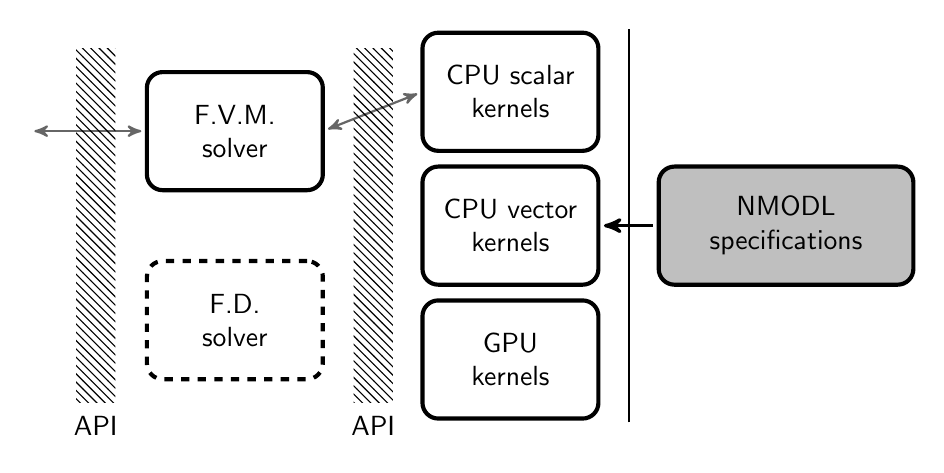
\begin{tikzpicture}[x=0cm, y=0cm, node distance=0 cm,outer sep = 0pt]
\tikzstyle{basicbox}=[draw=black, fill=white, rectangle, line width=1.5pt, rounded corners=2mm,
    minimum height=\nodeheight, minimum width=2cm, text width=2cm, anchor=west, align=center]
%
\tikzstyle{dashedbox}=[draw=black, fill=white, rectangle, line width=1.5pt, rounded corners=2mm,
    dashed, minimum height=\nodeheight, minimum width=2cm, text width=2cm, anchor=west, align=center]
%
\tikzstyle{nmodlbox}=[draw=black, fill=lightgray, rectangle, line width=1.5pt, rounded corners=2mm,
    minimum height=\nodeheight, minimum width=3cm, text width=3cm, anchor=west, align=center]
%
\tikzstyle{apibox}=[pattern=north west lines, rectangle,
                   minimum height=4.5cm, minimum width=0.5cm, align=center]

\node[basicbox] (fvm) at (0.0cm,1.2cm) {F.V.M.\\ solver};
\node[dashedbox] (fd) at (0.0cm,-1.2cm) {F.D. \\ solver};
\node[basicbox] (cpu)  at (3.5cm,1.7cm) {CPU scalar\\ kernels};
\node[basicbox] (cpuvector)  at (3.5cm,0cm) {CPU vector\\ kernels};
\node[basicbox] (gpu)  at (3.5cm,-1.7cm) {GPU\\ kernels};

\path[pil,<->] (-1.5cm,1.2cm) edge (fvm.west);
\path[pil,<->] (fvm.east) edge (cpu.west);

\node[apibox] (api2) at (-0.65cm,0cm) {};
\node[apibox] (api3) at (2.875cm,0cm) {};

\draw[thick] (6.125cm,-2.5cm) -- (6.125cm,2.5cm);

\node[nmodlbox] (nmodl) at (6.5cm,0cm) {NMODL\\ specifications};
\path[pil,<-,very thick,black] (cpuvector.east) edge (nmodl.west);

\node[align=center] [below = 0.05cm of api2] {API};
\node[align=center] [below = 0.05cm of api3] {API};

\end{tikzpicture}
\end{document}

